\documentclass[10pt]{article}
\usepackage[spanish]{babel}
\usepackage{graphicx}
\usepackage{tabularx} % para width table
\usepackage[left=1.5cm,top=2.4cm,right=2.1cm,bottom=3cm,bindingoffset=0.5cm]{geometry} % original[22 iz,24 arri]
\usepackage{multirow}
\graphicspath{{img/}{img2/}}
\usepackage{url}
\usepackage{amsmath}
\usepackage{hyperref} % Hipervinculos
\usepackage{ragged2e} % Alineación
\usepackage{amssymb} %therefore
\usepackage{float} %Here
\usepackage{listings}
\usepackage{mathrsfs,mathtools} 
\usepackage{pdfpages} %Incluir pdf
\usepackage{csvsimple} %%----------ARCHIVOS CVS


\newsavebox\foobox
\newlength{\foodim}
\newcommand{\slantbox}[2][0]{\mbox{%
        \sbox{\foobox}{#2}%
        \foodim=#1\wd\foobox
        \hskip \wd\foobox
        \hskip -0.5\foodim
        \pdfsave
        \pdfsetmatrix{1 0 #1 1}%
        \llap{\usebox{\foobox}}%
        \pdfrestore
        \hskip 0.5\foodim
}}
\def\Laplace{\slantbox[-.45]{$\mathscr{L}$}}



%% paquetes para esta práctica (aquí abajo)-------------------------------

\usepackage{titlesec}
\titleformat{\section}
{\normalfont\Large\bfseries \raggedright}{\thesection}{1em}{}


%% Preambulo configuraciones adicionales----------------------------------

\newcommand{\iu}{{i\mkern1mu}} % definicon nuevo comando
\addtolength{\jot}{1em} % espacio vertical ecuaciones


%% Cuerpo principal-------------------------------------------------------

\begin{document}
	
	\centering
	\begin{tabular}{ |	p{30 mm}|	p{61 mm}	|	p{33mm}	| p{43mm}	| } 
		\hline
		
		
		\multirow{4}{30mm}{\centering 
\includegraphics[scale=0.22]{logo}} &
		\multirow{4}{61mm}{\centering \textbf{ \textbf{Manual de prácticas del Laboratorio de Análisis de Sistemas y Señales}}}    & Código: & MADO-76 \\
		\cline{3-4}
		& &  Versión & 01 \\
		\cline{3-4}
		& & Página: & 77/97 \\ \cline{3-4}
		& & Sección ISO: & 8.3 \\ \cline{3-4}
		& & Fecha de emisión: & 28 de frebrero 2019 \\
		\hline
	\end{tabular}
\begin{tabular}{ |	c |	c	| } 
	
	\multirow{2}{65mm}{ \centering Facultad de ingeniería} &
	\multirow{2}{111mm}{\centering \textbf{ Area/Departamento: \\ Laboratorio de control y robótica}}   \\
	& \\ \hline
\end{tabular}
\begin{tabular}{|p{180mm}|}
	\multirow{1}{180mm}{ \centering La impresion de este documento es una copia no controlada }  \\ \hline \end{tabular} \\

\vspace{1cm}


{\centering \LARGE Práctica N◦5 Respuesta de Sistemas Dinámicos }

\vspace{1.5cm}

\begin{figure}[!h]
	\centering
	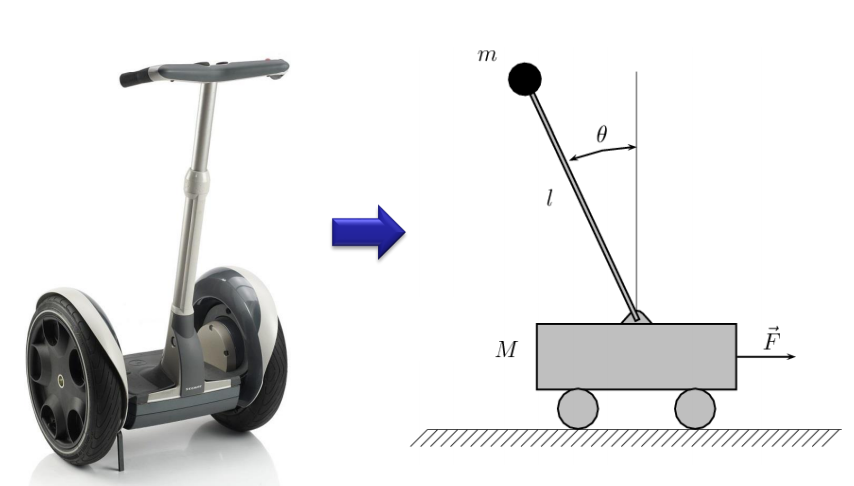
\includegraphics[scale=0.6]{portada.png}
\end{figure}

\hspace{2cm}

\hspace{1cm}
\begin{tabular}{|c| p{122mm}|}
	\hline
	\multirow{4}{50mm}{\\ \centering \large Apellidos y nombres}	 &  \\  
	& Alfaro Domínguez Rodrigo  \\  \cline{2-2}
	&  \\  
	& Barrera Peña Víctor Miguel \\  \cline{2-2}
	&  \\  
	& Villeda Hernández Erick Ricardo \\ 
	\hline
\end{tabular}
\begin{tabular}{|p{50mm} | c | p{80mm}| p{23mm} |}
	Grpo: & 4 & \multirow{2}{90mm}{Profesor: M.I Lauro Fernando Vazquez Alberto } & Calificación \\ \cline{1-2}
	Brigada: & 1 &  &\\ \hline
	Semestre: & 2021-1 & Fecha de ejecución: 29/09/2020 & \\ \hline
\end{tabular}





	\includepdf[pages={2-8}]{latex/practica4.pdf}
	\noindent \justifying

\section{Previo}

\subsection{Identificar un sistema dinámico que se tenga en casa y definir la salida y la entrada del mismo (para discusión en clase)}
\subsection{¿Como analizaría un sistema de orden mayor?}
Para analizar un sistema de orden superior empezamos por escribir su función de transferencia:
\begin{equation}
H(s)=K\frac{(s-z_1)(s-z_2)...(s-z_n)}{(s-p_1)(s-p_2)(s-p_n)}
\end{equation} 
La mayor parte de la información de como funciona el ssitema nos la darán la localización de los polos y ceros. Esto determina si el sistema es estable o no.\\
En caso de tener polos reales la ecuación toma la siguiente forma:
\begin{equation}
H(s)=\frac{a_1}{s-p_1}+...+\frac{a_n}{s-p_n}
\end{equation}
A partir de aquí analizamos su respuesta a un impulso y un escalón, quedándonos sus ecuaciones de una de las siguientes formas respectivamente:
\begin{equation}
y_{imp}=\alpha_1 e^{p_1t}+..+\alpha_n e^{p_nt}
\end{equation}
\begin{equation}
y_{step}=\beta_0 + \beta_1 e^{p_1t}+...+ \beta_n e^{p_nt}
\end{equation}
Cada polo real p genera un término exponencial en la respuesta. El comportamiento de las osilaciones va a depender de si la parte real del poplo es negativa o positiva, mientras que la magnitud depende de los ceros.\\
En el caso de un sistema de segundo orden podemos escribir su ecuación característica en términos de zeta y omega, de la siguiente forma:
\begin{equation}
\frac{d^2y(t)}{dt^2}+2\zeta \omega_n \frac{dy(t)}{dt}+(\omega_n)^2y(t)=k(\omega_n)^2x(t)
\end{equation}
A partir de su respuesta en la ecuación homogénea podemos llegar a un polinimio de la siguiente forma:
\begin{equation}
s^2+2\zeta\omega_ns+\omega^2_n=0
\end{equation}
La respuesta del sistema va a depender de los valores que tenga el término $\zeta$, siendo sus valores posibles entre cero e infinito positivo. Lo que nos interesará para el diseño de un sistema es que su valor sea mayor o igual a uno.
\subsection{¿Cuál es la importancia de la constante de tiempo $\tau$ y el factor de amortiguamiento $\zeta$ ?}


	\includepdf[pages={9}]{latex/practica4.pdf}
	%act1
	\subsection{Solución actividad 1}
\noindent \textbf{Actividad 1}\\
En la Figura 28 se muestran 5 sistemas diferentes, de los cuales se deben identificar las variables f´ısicas,
los elementos almacenadores de flujo, de esfuerzo, disipadores y fuentes de energ´ıa, una vez identificados los
sistemas, llenar la tabla mostrada en la Figura29.\\

\begin{center}
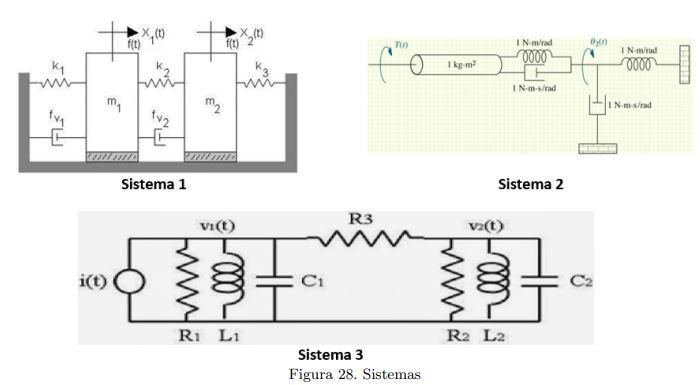
\includegraphics[scale=0.6]{img1.jpg} 
\end{center}

\begin{table}[t]
\begin{center}
\begin{tabular}{| c | c | c | c | }

\hline
Actividad & Sistema 1 & Sistema 2 & Sistema 3 \\ \hline
Tipo & mecánico translacional. & mecánico rotacional. & eléctrico. \\ \hline
& x & $\theta$ & v \\ 
Variables físicas  & v & $\omega$ & i \\ 
& a & $\alpha$ &  \\ \hline

Almacenadores de flujo & m$_{1}$ & m$_{1}$ & C$_{1}$ \\
& m$_{2}$ &  & C$_{2}$ \\ 
& $\dot{x}=\frac{p}{m}[kg]$ & $\omega=\frac{H}{I}[Nms^{2}]$ & $i=\frac{\lambda}{L}[Vs/A]$ \\
&  &  &  \\
Leyes de c. general& $a=\frac{1}{m}\frac{d}{dt}p$ & $\alpha=\frac{1}{J}\frac{d}{dt}h$ & $i_{c}=C\frac{d}{dt}VC$ \\ \hline

& k$_{1}$ & k$_{1}$ & L$_{1}$ \\ 
Almacenadores de esfuerzo & k$_{2}$ & k$_{2}$ & L$_{2}$ \\ 
& k$_{3}$ &  &  \\
& $F=Kx[N/m]$ & $\tau=K_{\omega}\omega[Nm/rad]$ & $e=\frac{q}{C}[As/V]$ \\
&  &  &  \\
Leyes de c. general& $f_{12}=Kx_{12}$ & $\tau=K_{\theta}\theta_{12}$ & $V_{L}=L\frac{d}{dt}iL$ \\ \hline

fuentes de energía & f$_{1}$(t) & $\tau$ & i \\ 
& f$_{2}$(t) &  &  \\ \hline

Elementos disipadores & fv$_{1}$ & f$\omega$ $_{1}$ & R$_{1}$ \\
& fv$_{2}$ & f$\omega$ $_{2}$ & R$_{2}$ \\
&  &  & R$_{3}$ \\ 
& $F=b\dot{x}[Ns/m]$ & $\tau=b_{\omega}\theta[Nms]$ & $e=Ri[\Omega]$ \\
&  &  &  \\
Leyes de c. general& $f_{12}=Kx_{12}$ & $\tau=K_{\theta}\theta_{12}$ & $V_{L}=L\frac{d}{dt}iL$ \\ \hline


\end{tabular}
\caption{Figura 29. Identificación de sistemas físicos.}
\end{center}
\end{table}
	\includepdf[pages={10}]{latex/practica4.pdf}
	%act2-3
	\subsection{Solución actividad 2}
Diagrama de cuerpo libre:\\
\begin{center}
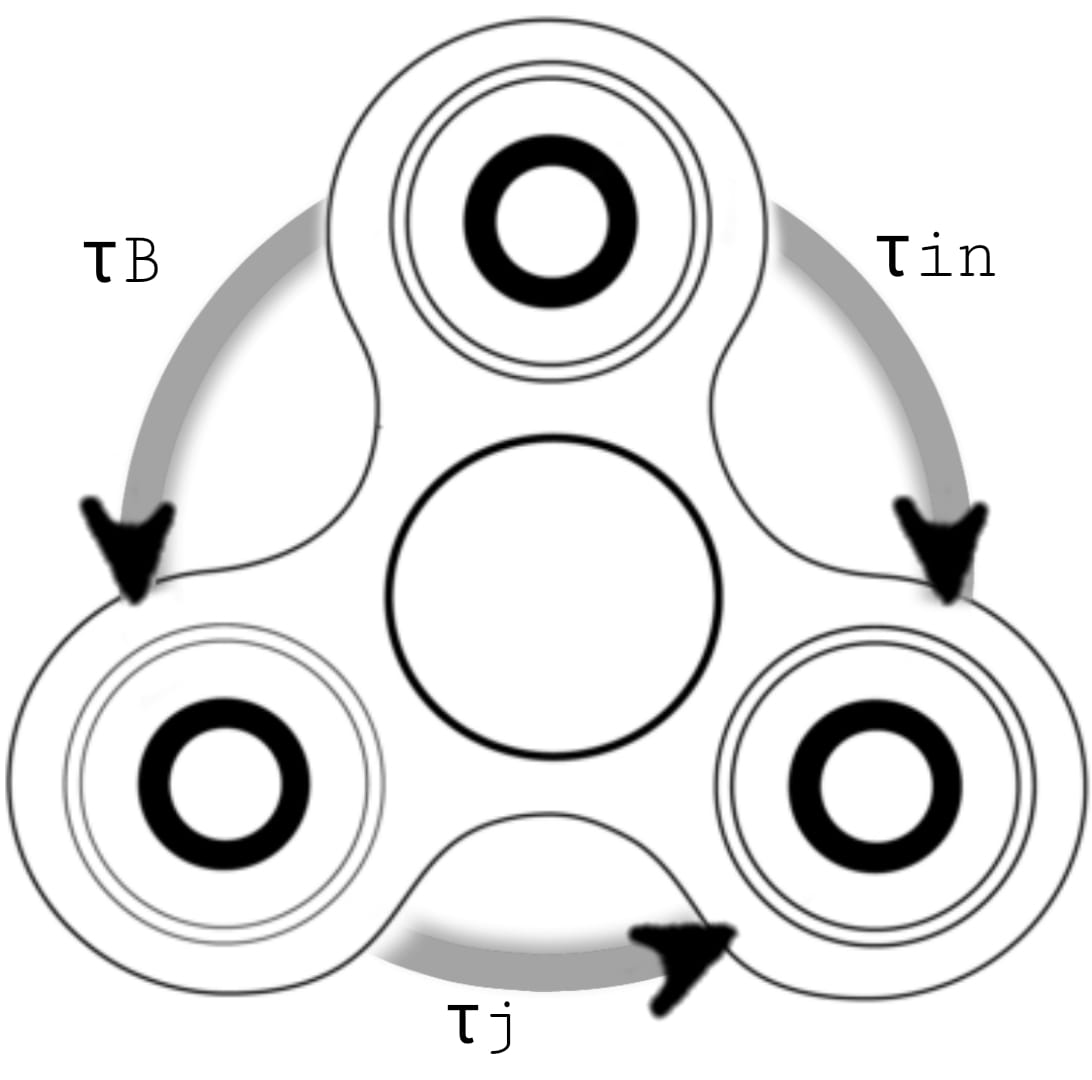
\includegraphics[scale=0.15]{DCL.jpeg} \\
\end{center}
Sistema mecánico rotacional.\\
$\tau_{in}=$Fuente de energía(Fuerza de entrada).\\
$\tau_{j}=$Masa(Inercia).\\
$\tau_{B}=$Disipador(Fricción).\\
$$\tau_{in}=\tau_{j}+\tau_{B}$$
Donde: $\tau_{j}=J\alpha,\alpha=\dot{\omega}$ y $\tau_{B}=B\omega$\\
$\alpha=\dot{\omega}=$primera derivada de la posición angular.
$$\tau_{in}=J\dot{\omega}+B\omega$$
$$\tau_{in}=J\ddot{\theta}+B\dot{\theta}$$
\textbf{Modelo matemático del sistema: $\tau_{in}=J\ddot{\theta}+B\dot{\theta}$}\\

\begin{center}
	\csvautotabular{latex/tabla.csv}
\end{center}

\subsection{Solución actividad 3}

Diagrama eléctrico equivalente:\\
\begin{center}
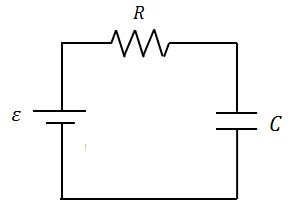
\includegraphics[scale=0.7]{ACT3.png} 
\end{center}
Donde: Capacitor(C)=masa=$\tau_{j}$, Resistencia(R)=disipador=$\tau_{B}$, Fuente de energía($\epsilon$)=$\tau_{in}$.
\end{document}


	\includepdf[pages={11}]{latex/practica4.pdf}
	%act4
	\subsection{Solución actividad 4}
	\includepdf[pages={12}]{latex/practica4.pdf}
	%act5
	\subsection{Solución actividad 5}
1. Identificar el numero de elementos que almacenan energía:\\
El sistema presenta cuatro almacenadores de energía. La ecuación resultante va a ser de orden dos, debido a que el sistema presenta los dos tipos de elementos almacenadores (de flujo y de esfuerzo), siendo estos elementos los siguientes:\\
\begin{itemize}
\item Almacenadores de esfuerzo: Inductores L y Lm
\item Almacenadores de flujo: Capacitor C y la masa rotada.
\end{itemize}
2. Identificar el número de restricciones físicas tanto de compatibilidad como de continuidad.\\
El sistema presenta cuatro restricciones físicas y se dividen de la siguiente forma: los dos circuitos en serie presentan restricciones de compatibilidad, mientras que la conexión en paralelo y la masa presentan restricciones de tipo de compatibilidad.\\
3. Plantear las restricciones físicas encontradas:\\
De la primera malla obtenemos el siguiente análisis:\\
\begin{equation}
E=V_L+v
\end{equation}
Si analizamos uno de los nodos que conecta a la primera malla con la conexión en paralelo obtenemos:\\
\begin{equation}
i=i_c+i_r+i_a
\end{equation}
De la segunda malla obtenemos el siguiente análisis:
\begin{equation}
v=V_{RM}+V_{LM}+VM
\end{equation}
Y por último, del sistema de la masa obtenemos lo siguiente:
\begin{equation}
K_{ew}=J\frac{d}{dt}w+Bw-J_L
\end{equation}
4. Sustituir las relaciones constitutivas de los elementos
Sustituyendo las relaciones constitutivas de los elementos de la primera malla obtenemos:
\begin{equation}
E=L\frac{d}{dt}i(t)+w
\end{equation}
En cuanto a los elementos constitutivos del análisis de la entrada de corriente al nodo alfa queda:
\begin{equation}
i=C\frac{dv}{dt}+\frac{v}{R}+i_a
\end{equation}
Y finalmente podemos expresar el análisis de la segunda malla de la siguiente forma:
\begin{equation}
v=R_mi_a+L_m\frac{d}{dt}i_a+K_{ew}
\end{equation}
5. Obtener el modelo matemático de forma matricial.
La representación del modelo matemático en forma matricial responde a la siguiente forma:
\begin{equation}
x'(t)=A(y)x(t)+B(t)u(t)
\end{equation}
La cual la podemos denotar como:
\begin{equation}
x'=Ax+Bu
\end{equation}
Donde $x'$ es el vector de variables de estados, $A$ es la matriz de estados, $x$ es el vector de estados, $B$ es la matriz de entrada y $u$ es el vector de entrada.\\
Para poder usar la expresión anterior debemos de dejar las ecuaciones de las restricciones de nuestro sistema en función de sus derivadas normalizadas. Po lo cual las ecuaciones a usar quedarán de las siguientes:
\begin{equation}
i'=-\frac{1}{L}v+\frac{1}{L}E
\end{equation}
\begin{equation}
v'=\frac{1}{C}i-\frac{1}{RC}v-\frac{1}{C}i_a
\end{equation}
\begin{equation}
i'_a=\frac{1}{L_m}v-\frac{1}{L_m}R_mi_a-\frac{K_e}{L_m}w
\end{equation}
\begin{equation}
w'=\frac{1}{J}k_ei_a-\frac{1}{J}B_w
\end{equation}
Ya teniendo las ecuaciones despejadas podemos sustituir en la ecuación matricial obteniendo la siguiente expresión:\\
llflfld
\begin{equation}
\begin{pmatrix}
i'\\
v'\\
i_a'\\
w' 
\end{pmatrix}
=
\begin{pmatrix}
0 & -\frac{1}{L} & 0 & 0\\
\frac{1}{C} & -\frac{1}{RC} & -\frac{1}{C} & 0\\
0 & \frac{1}{L_m} & -\frac{R_m}{L_m} & \frac{K_e}{L_m}\\
0 & 0 & \frac{K_e}{J} & -\frac{B}{J}
\end{pmatrix}
\begin{pmatrix}
i\\
v\\
i_a\\
w
\end{pmatrix}
+
\begin{pmatrix}
\frac{1}{L}\\
0\\
0\\
0\\
\end{pmatrix}
E
\end{equation}
6. ¿Qué se puede concluir del sistema físico obtenido?//
Que la unión de distintos sistemas físicos nos da como resultado la unión de las ecuaciones de dichos sistemas, es decir, su modelo matemático va a ser la suma de los modelos matemáticos de cada uno de los subsistemas que conforman a dicho sistema.

\section{OBSERVACIONES Y CONCLUSIONES}

	Villeda Hernandez Erick Ricardo: En la realización de esta práctica aplicamos los conocimientos teóricos de sobre el modelado de sistemas físicos (eléctricos, mecánicos translacional y mecánicos rotacionales), los cuales nos ayudaron a conocer y a diferenciar los elementos principales de todo sistema físico como los almacenadores de flujo, esfuerzo, los disipadores y la fuente de energía.Ya que dependiendo del tipo de sistemas con el que estemos trabajando va a variar su elementos. Se trabajó parte del funcionamiento de un sistema híbrido y se analizaron  las restricciones de constitución, continuidad, y compatibilidad para poder obtener un modelo matemático más apegado a la realidad.

	\nocite{webNijtEdu}
	\nocite{*}
	\bibliographystyle{plain}
	\bibliography{latex/referencias.bib}
\end{document}

